\chapter{Referencial Teórico}
Este capítulo tem como objetivo fornecer os principais conceitos relacionados aos temas: alinhamento estratégico e planejamento de TI. Também é abordado o planejamento de TI no contexto do setor público e seus instrumentos normativos. Por fim, são apresentados detalhes do instrumento de planejamento alvo desta pesquisa, o Plano Diretor de Tecnologia da Informação.

\section{Alinhamento Estratégico}

% sobre estratégia de TI
As organizações necessitam cada vez mais dos Sistemas de Informação (SI) e TI para apoiar a tomada de decisões \cite{rezende:08}. \citeonline{boynton:90} definem estratégia de TI como o conjunto de atividades voltadas para (i) reconhecer oportunidades organizacionais para a utilização de tecnologia da informação; (ii) determinar as necessidades de recursos para explorar as oportunidades; (iii) o desenvolvimento de planos de ação para a execução das oportunidades e para atender as necessidades de recursos. Para \citeonline{earl:89}, estratégia de TI é o plano direcional que decide o que fazer com a TI de uma organização a longo prazo. 

% conceito de alinhamento estratégico de pelo menos dois autores fodas 
A estratégia de TI não lida somente com tecnologia. A estratégia de TI envolve criar ambientes integrados que aumentam a efetividade dos recursos humanos, processos de negócio, estruturas organizacionais e tecnologias de modo a transformar a posição competitiva do negócio \cite{luftmanetal:04}. Alinhamento estratégico, ou alinhamento estratégico de TI, diz respeito à forma com que a estratégia de TI está alinhada ao negócio e como o negócio pode ou deveria estar alinhado com a TI \cite{luftman:04}. 

\begin{figure}[h!]
\centering % para centralizarmos a figura
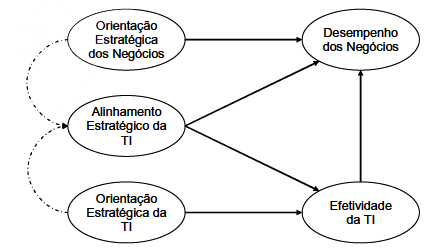
\includegraphics[width=10cm]{figuras/modeloChan.png}
\caption{Modelo de alinhamento estratégico de \citeonline{chan:97}}
\label{figura:modeloChan}
\end{figure}


No modelo de alinhamento estratégico de \citeonline{chan:97}, representado na Figura \ref{figura:modeloChan}, fica explícito que o alinhamento estratégico de TI é composto pela estratégia do negócio e pela estratégia de TI. Além disso, este autor destaca que o alinhamento estratégico é o melhor indicador da efetividade da TI e também do desempenho organizacional.

A estratégia global da organização, dita estratégia do negócio, e as estratégias de TI devem estar alinhadas, ou seja, deve haver harmonia entre as metas e planos de implementação de TI com as metas e a estrutura da organização \cite{luftmanetal:04}. \citeonline{henderson:99} criaram um modelo, representado na Figura \ref{figura:modeloHenderson}, no qual o alinhamento estratégico é apresentado como a adequação e integração funcional entre ambiente externo (mercado) e interno (estrutura organizacional, recursos financeiros, tecnológicos e humanos) para desenvolver as competências e maximizar o desempenho da organização. 

\begin{figure}[h!]
\centering % para centralizarmos a figura
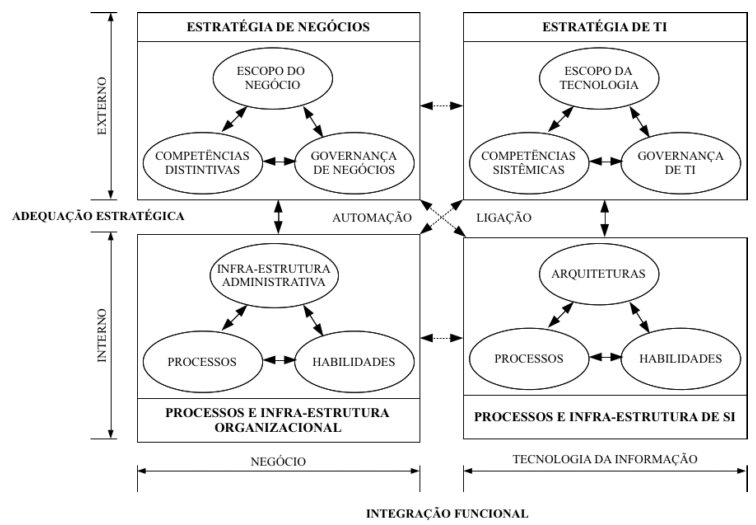
\includegraphics[width=14cm]{figuras/modeloHenderson.png}
\caption{Modelo de alinhamento estratégico de \citeonline{henderson:99}}
\label{figura:modeloHenderson}
\end{figure}

\citeonline{king:88} e \citeonline{chan:97} abordam o alinhamento estratégico sob o ponto de vista dos documentos de planejamento da organização e da área de TI: plano estratégico de negócio (PEN) e o plano estratégico de TI (PETI). Desta forma, o alinhamento estratégico trata-se do alinhamento entre o PEN e o PETI, ou seja, os objetivos presentes no PETI devem estar direcionados ao atendimento dos objetivos organizacionais presentes no PEN.

As empresas que conseguem alinhar suas estratégias de negócio com as estratégias de TI atingem aumento de desempenho em seus negócios \cite{chan:06}. A importância estratégica da TI na gestão de organizações é destacada no \textit{ranking} de preocupações de gestores, no qual o alinhamento estratégico de TI se encontra como preocupação número um nas publicações de 2013, 2014 e, recentemente, em pesquisa de 2015, ficando à frente de temas como segurança/privacidade, produtividade e inovação  \cite{kappelman:15}. Pesquisas tanto da área de TI quanto da área de administração evidenciam o impacto positivo do alinhamento das estratégias de TI com o negócio \cite{reich:96,luftman:96,sabherwal:01};

\citeonline{cragg2002alignment} realizou um estudo com 250 pequenas empresas do Reino Unido e constatou que as empresas que possuem alto índice de alinhamento entre a área de TI e os objetivos da empresa, obtiveram melhor desempenho organizacional do que as empresas com baixo alinhamento estratégico. Neste estudo, por se tratar de pequenas empresas, o alinhamento estratégico foi mensurado avaliando o quanto a TI fornecia apoio à determinadas estratégias de negócio, tais como estratégia de preço, estratégia de qualidade de produto e estratégia de diferenciação no mercado. O resultado da pesquisa verificou que quanto mais presente a TI era nestas estratégias das empresas, melhor era o desempenho das mesmas.

\section{Planejamento de TI}

Existem diversos termos utilizados por diferentes autores que remetem ao planejamento de TI, tais como plano estratégico de sistemas de informação (PESI), plano estratégico de tecnologia da informação (PETI) e plano diretor de tecnologia da informação (PDTI) \cite{rezende:08}. \citeonline{barros:13} realizou um mapeamento de diferentes conceitos e denominações de planejamento de TI, alguns destes conceitos são apresentados na Tabela \ref{tabela:conceitosPlanos}.

% Please add the following required packages to your document preamble:
% \usepackage{graphicx}
% \usepackage[table,xcdraw]{xcolor}
% If you use beamer only pass "xcolor=table" option, i.e. \documentclass[xcolor=table]{beamer}
\begin{table}[h!]
\centering
\resizebox{\textwidth}{!}{%
\begin{tabular}{|l|l|}
\hline
\rowcolor[HTML]{9B9B9B} 
\multicolumn{1}{|c|}{\cellcolor[HTML]{9B9B9B}\textbf{Denominação}}       & \multicolumn{1}{c|}{\cellcolor[HTML]{9B9B9B}\textbf{Conceito}}                                                                                                                                                                                                                                    \\ \hline
\begin{tabular}[c]{@{}l@{}}Planejamento\\ Estratégico de SI\end{tabular} & \begin{tabular}[c]{@{}l@{}}É o processo de identificar um portfólio de aplicações baseadas em \\ computadores para apoiar a organização na execução do seu plano de \\ negócios e,consequentemente, na realização dos seus objetivos \\ organizacionais \cite{earl:89}.\end{tabular}           \\ \hline
Planejamento de SI/TI                                                    & \begin{tabular}[c]{@{}l@{}}Um conjunto de metas de longo prazo que descrevem a infraestrutura de\\ TI e iniciativas principais de SI necessárias para alcançar as metas da \\ organização \cite{turban:01}.\end{tabular}                                                                       \\ \hline
Plano Estratégico de TI                                                  & \begin{tabular}[c]{@{}l@{}}Plano de longo prazo, ou seja, com horizonte de três a cinco anos, no qual \\ as direções de negócios e de TI descrevem de forma colaborativa como os \\ recursos de TI contribuirão com o objetivos estratégicos da organização \\ \cite{itCobit:07}.\end{tabular} \\ \hline
Plano Diretor de TI                                                      & \begin{tabular}[c]{@{}l@{}}Instrumento de diagnóstico, planejamento e gestão dos recursos e processos\\ de TI que visa atender às necessidades tecnológicas e de informação de um \\ órgão ou entidade para um determinado período \cite{in04:08}.\end{tabular}                                   \\ \hline
\end{tabular}%
}
\caption{Conceitos de planejamento de TI, adaptado de \citeonline{barros:13}}
\label{tabela:conceitosPlanos}
\end{table}

Atualmente, a maioria das organizações acreditam que as decisões ligadas à tecnologia devem ser tomadas com uma compreensão clara da direção e estratégia de negócios da organização \cite{pollack:10}. Na prática, um plano estratégico indica onde a organização quer chegar e como ela pretende chegar neste objetivo, tal plano deve apresentar uma visão de futuro que orienta a tomada de decisões do presente \cite{mcnurlin:09}. 

De acordo com \citeonline{pereira:07}, o processo de planejamento estratégico de uma organização pode ser dividido em três momentos: (i) diagnóstico estratégico; (ii) definição das etapas do planejamento; (iii) implementação e controle do processo de planejamento estratégico. Fazendo um paralelo com estes três momentos, o planejamento de TI também apresenta o momento de diagnóstico estratégico de TI (alinhamento estratégico), o momento de elaboração do planejamento de TI e, por fim, o momento de implementação e controle do processo de planejamento de TI \cite{paula:12}.

Para \citeonline{ward:16}, o planejamento estratégico da área de tecnologia de uma organização pode abordar a estratégia de sistemas de informação e a estratégia de tecnologia da informação. Enquanto a estratégia de sistemas de informação define e prioriza os investimentos necessários às aplicações ideais que suportam as demandas da organização, a estratégia de tecnologia da informação busca prover os serviços e recursos de TI (hardware, software e telecomunicações). 

 \begin{citacao}
O planejamento estratégico de SI/TI busca identificar, avaliar, planejar informações, conhecimentos organizacionais e soluções de tecnologia para dar suporte às decisões e às ações previstas para cada um dos objetivos estratégicos identificados nos planos estratégicos e aborda, quase sempre, elementos como: processos, tecnologia, pessoas e seus relacionamentos \cite[p. 22]{teixeira:10}.
 \end{citacao}

\citeonline{ward:16} propõem um modelo de planejamento estratégico de SI/TI baseado em entradas, processamento e saídas. As entradas do modelo são as seguintes:

\begin{itemize}
\item \textbf{Ambiente interno de negócio}: estratégia de negócio, objetivos, recursos, processos, cultura e valores organizacionais;
\item \textbf{Ambiente externo de negócio}: ambiente econômico e competitivo onde a empresa atua;
\item \textbf{Ambiente interno de TI}: a perspectiva da TI no negócio, sua maturidade, cobertura no negócio, contribuição para os objetivos do negócio, capacidade, recursos, infraestrutura tecnológica, portfólio de aplicações e serviços;
\item \textbf{Ambiente externo de TI}: tendências tecnológicas e oportunidades, como a TI de outras empresas utilizam a tecnologia, principalmente clientes, concorrentes e fornecedores.
\end{itemize}

As saídas produzidas de acordo com o modelo de planejamento estratégico de SI/TI de \citeonline{ward:16}, são:
\begin{itemize}
\item \textbf{Gerenciamento de estratégia de TI}: elementos comuns da estratégia que se aplicam em toda a organização, garantindo a coerência das políticas onde necessário;
\item \textbf{Estratégia de SI do negócio}: como cada unidade ou função irá implantar a TI na realização dos seus objetivos de negócios;
\item \textbf{Portfólio de aplicações}: ao lado de cada um dos objetivos do negócio estão portfólios de aplicações a serem desenvolvidas para a unidade de negócio e modelos de negócios, descrevendo as arquiteturas de informação de cada aplicação. Isto pode incluir como ela vai ser usada em alguma data futura para ajudar as unidades de alcançar os seus objetivos;
\item \textbf{Estratégia de TI}: políticas e estratégias para a gestão de tecnologia e de recursos especializados.
\end{itemize}


O modelo de \citeonline{ward:16} foi criado para organizações que visam utilizar a TI para obter vantagem competitiva em mercados altamente disputados. Outros modelos são abordados por \citeonline{teixeira:10}, destacando os modelos: \cite{nolan:73}, \cite{sullivan:85}, \cite{teo:97}, \cite{mentzas:97}, \cite{cassidy:98}, \cite{min:99}, \cite{gordon:06} e \cite{newkirk:07}. Diante da variedade de modelos e de estudos sobre o planejamento estratégico de sistemas de informação, \citeonline{brown:04} utilizaram o método \textit{Grounded Theory} para elaborar uma teoria abrangente baseada na literatura científica. Esta teoria é ilustrada pelo diagrama da Figura \ref{figura:modeloBrown}.

\begin{figure}[h!]
\centering % para centralizarmos a figura
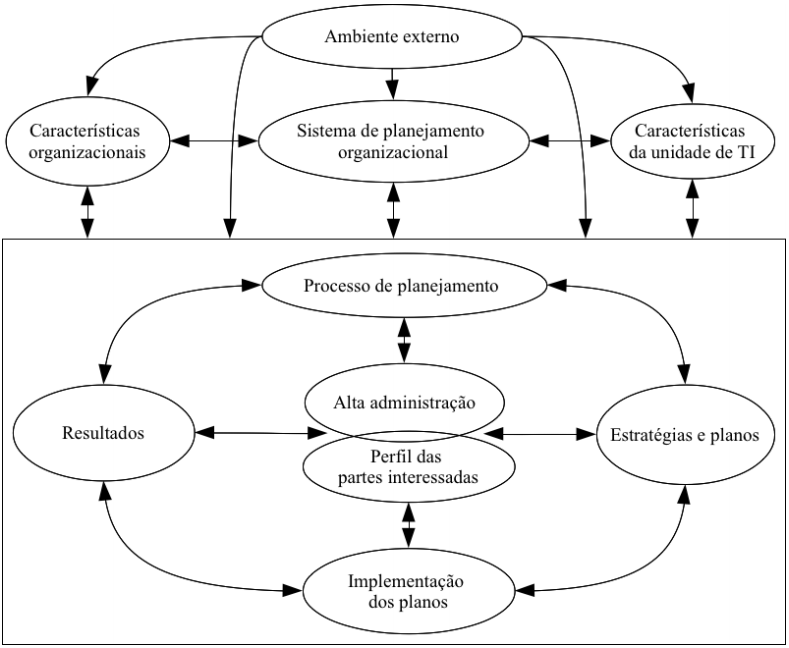
\includegraphics[width=14cm]{figuras/modeloBrown.png}
\caption{Modelo teórico de \citeonline{brown:04}, extraído de \citeonline{barros:13}}
\label{figura:modeloBrown}
\end{figure}

O modelo teórico de \citeonline{brown:04} exibe, através das categorias mapeadas na pesquisa, os conceitos que permeiam o planejamento de TI e suas relações. As categorias apresentadas neste modelo são:
\begin{itemize}
\item Ambiente externo;
\item Características organizacionais;
\item Sistema de planejamento organizacional;
\item Características da unidade de TI;
\item Processo de planejamento;
\item Resultados;
\item Alta administração;
\item Perfil das partes interessadas;
\item Estratégias e planos;
\item Implementação dos planos.
\end{itemize}


A presente pesquisa está inserida no contexto de organizações públicas. Desta forma, os modelos de planejamento voltados para organizações que disputam mercado podem não ser totalmente aplicáveis no cenário do setor público, apesar de apresentarem conceitos que podem ter correspondência no ambiente organizacional público. Diante disso, na seção seguinte são apresentados conceitos e abordagens de planejamento de TI voltados para obter eficiência e eficácia operacional, ou seja, objetivos mais aderentes à organizações públicas.

\section{Planejamento de TI no Setor Público}
% Luiza Página 27

% mundo
%ver minha revisão da literatura se tem nos artigos gringos umas referências sobre o planning na gringa

Espera-se de entidades públicas, que se dedicam à prestação de serviços públicos, o exercício das suas funções em níveis de qualidade comparáveis ao setor privado \cite{nezakati:14}. A denominação de planejamento de TI mais comum em bases acadêmicas estrangeiras é o planejamento de sistemas de informação (\textit{strategic information systems panning}). As agências estatais que se dedicam ao planejamento estratégico de sistemas de informação, de maneira formal e abrangente, são capazes de promover um ambiente mais favorável à utilização de TI dentro do governo \cite{bajjaly:98}. Casos de sucesso da aplicação de planejamento de TI no setor privado sugerem que adaptações nos modelos tradicionais de planejamento de TI podem preencher a lacuna entre os recursos estatais e as necessidades dos cidadãos \cite{dufner:02}.

% Can Private Sector Strategic Information Systems Planning Techniques Work for the Public Sector?
\citeonline{dufner:02} realizaram uma pesquisa com órgãos governamentais dos Estados Unidos e destacou que entidades do poder executivo e legislativo dos estados tinham baixo índice de envolvimento com planejamento de TI. Nesta pesquisa os autores buscam evidências de que o modelo criado para o planejamento estratégico de sistemas de informação é originalmente voltado para entidades privadas e vários fatores demandam adaptação no modelo para o setor público, por exemplo os objetivos organizacionais. A pesquisa de \citeonline{dufner:02} mostra que os objetivos organizacionais das empresas privadas abordam questões relacionadas à TI em suas metas, enquanto em empresas públicas a TI figura como uma ferramenta auxiliar e não como um componente importante para atingir os objetivos da organização. 

\citeonline{abu:09} traz um estudo sobre diferenças entre planejamento estratégico de sistemas de informação de empresas privadas e públicas, além de apresentar fatores de sucesso para um modelo de planejamento de TI voltado ao setor público. Em \citeonline{dufner:05}, os autores analisam quatro modelos de planejamento de TI utilizados em instituições públicas dos Estados Unidos. 

Com relação aos modelos de planejamento de TI para o setor público brasileiro, \citeonline{rezende:07} propôs uma metodologia para o planejamento de informação, conhecimento e informática para entidades públicas municipais. \citeonline{fagundes:11} propõe um modelo para elaboração do PDTI baseado em arquitetura corporativa e governança de TI. Em 2012, o Sistema de Administração dos Recursos de Tecnologia da Informação (SISP) do governo federal publicou a primeira versão do guia de elaboração do PDTI \cite{sisp:12}. %Na seção 3.3.4 deste trabalho são apresentados os principais modelos dedicados ao PDTI.

Assim como empresas privadas, os órgãos da administração pública necessitam planejar ações para atingir suas metas. A própria Constituição da República Federativa do Brasil de 1988, em seu artigo 174, declara que o Estado, como agente regulador da economia, exercerá a função de planejamento \cite{cf:88}. Na Administração Pública Federal o planejamento é um princípio fundamental estabelecido no Decreto Lei 200/1967. Desde 2008, através da Instrução Normativa 04/2008 \cite{in04:08} e da Estratégia Geral de Tecnologia da Informação \cite{egti:08}, os órgãos do poder executivo federal são obrigados a planejar as ações de TI através do PDTI. Portanto, todas as organizações públicas, devem desenvolver processos de planejamento e de monitoramento nos níveis institucionais e na área de TI \cite{tcuManual:07}.  

É importante que os órgãos públicos possuam planos, nos níveis estratégico, tático e/ou operacional, para as funções financeira, logística e de TI. O PETI, situado no nível estratégico, é um documento que complementa o Plano Estratégico Institucional, por meio do planejamento dos recursos de TI, possibilitando a definição de objetivos específicos para a área de TI. Ele estabelece as diretrizes e as metas que orientam a construção do planejamento de TI do órgão. Já no nível tático, o instrumento mais comumente usado para representar o planejamento de TI é o PDTI. O PDTI descreve de forma tática como uma organização, no que se refere à tecnologia da informação, pode realizar a transição de uma situação atual para uma situação futura, a partir da definição de um plano de metas e ações. No nível operacional, os planos de ação auxiliam a execução das ações e o alcance das metas, alinhados ao PDTI \cite{sisp:15}. 

É relevante compreender o fluxo dos processos de planejamento do governo federal brasileiro que se relacionam com os processos de planejamento de TI dos órgãos. O planejamento do governo é materializado em três instrumentos: Plano Plurianual (PPA), a Lei de Diretrizes Orçamentárias (LDO) e a Lei Orçamentária Anual (LOA). Os órgãos, por sua vez, tem como principal instrumento de planejamento o Planejamento Estratégico Institucional (PEI), alinhado aos planos superiores. Os setores de TI dos órgãos podem possuir o PETI e o PDTI como instrumentos de planejamento da área de tecnologia da informação, sendo que estes devem estar alinhados ao PEI \cite{sisp:15}. Segundo a IN 04/2014, ``inexistindo o plano estratégico institucional, sua ausência deverá ser registrada no PDTI e deverá ser utilizado um documento equivalente, como o Plano Plurianual'' \cite{in04:14}. A Figura \ref{figura:fluxoPlanejamentoGov} ilustra a relação dos instrumentos de planejamento de TI com os instrumentos de planejamento do governo.

\begin{figure}[h!]
\centering % para centralizarmos a figura
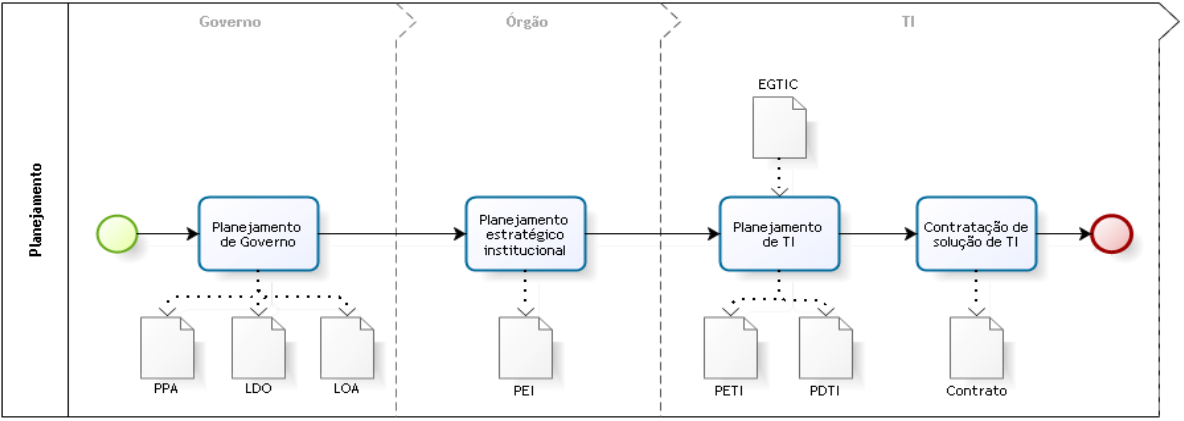
\includegraphics[width=14cm]{figuras/fluxoPlanejamentoGov.png}
\caption{Fluxo dos processos de planejamento de TI no governo brasileiro, extraído de \citeonline{sisp:15}.}
\label{figura:fluxoPlanejamentoGov}
\end{figure}

\subsection{IN 04/2008}

De acordo com balanço de compras públicas de 2014, o governo federal movimentou R\$6,03 bilhões com aquisições de bens e serviços de tecnologia da informação e comunicação \cite{balanco:14}. Isto evidencia que o setor público brasileiro é um grande cliente de serviços de TI. Segundo \citeonline{cruz:08}, ``o aumento na frequência de acórdãos e decisões do TCU relacionados no âmbito das contratações de serviços de TI, em especial a partir de 2002, indica maior preocupação do TCU com o tema e sugere a existência de problemas de gestão de contratação de serviços neste setor''. No Acórdão 786/2006 do TCU, itens 68 a 70 do voto do relator, são indicados recorrentes problemas em contratações de serviços de TI, além de críticas ao modelo de contratação da época:
\begin{citacao}
68.	Pode-se dizer que o modelo de contratação antes adotado pelo MDIC consistia na reunião de todos os serviços de informática do órgão em um único e grande contrato, adjudicado a uma única empresa, com pagamentos realizados por hora-trabalhada. 
69.	É necessário que se esclareça que essa prática, que equivale à contratação dos serviços de um CPD completo e terceirizado, não se restringia ao Ministério do Desenvolvimento, Indústria e Comércio Exterior. Em diversos processos examinados pelo Tribunal, verificou-se que foram muitos os casos em que licitações de serviços de informática vinham sendo promovidas pela Administração Pública Federal sem que se procedesse à divisão do objeto em parcelas, como preconizado pelo art. 23, §§ 1º e 2º, da Lei 8.666/93, apesar de tal alternativa se mostrar viável. A título de exemplo, podem ser citados certames realizados pelo Ministério do Planejamento (Concorrência 14/2000 - Decisão 1.067/2002 - Plenário), Agência Nacional do Cinema (Concorrência 02/2003 - Acórdão 1.937/203 - Plenário), Ministério da Educação (Concorrência 01/1999 - Acórdão 2.561/2004-2ª Câmara), Ministério da Justiça (Concorrência 03/2000 - Decisão 351/2002 - Plenário), entre outros.
70.	Esse modelo apresentava uma série de desvantagens potencialmente causadoras de prejuízos aos cofres públicos e à atividade da Administração. 
\end{citacao}

Diante de fatos desta natureza, o TCU recomendou, no mesmo acórdão (item 9.4), que Secretaria de Logística e Tecnologia da Informação (SLTI) do Ministério do Planejamento, Orçamento e Gestão elaborasse um modelo de licitação e contratação de serviços de TI para a APF:
\begin{citacao}
9.4. recomendar à Secretaria de Logística e Tecnologia da Informação do Ministério do Planejamento, Orçamento e Gestão que, a partir das diretrizes expostas na seção III do voto antecedente e nos Acórdãos deste Tribunal, sobretudo os de número 667/2005, 2.103/2005, 2.171/2005 e 2.172/2005, todos do Plenário, elabore um modelo de licitação e contratação de serviços de informática para a Administração Pública Federal e promova a implementação dele nos diversos órgãos e entidades sob sua coordenação mediante orientação normativa, que deve conter no mínimo:
9.4.1. a divisão dos serviços de informática necessários aos órgãos e entidades em tantos itens quanto sejam tecnicamente possíveis e suficientes;
9.4.2. a realização de licitação independente para cada item, contemplando requisitos de habilitação e critérios de avaliação de proposta técnica objetivos, relevantes e específicos para cada item, favorecendo assim a competitividade do certame, a redução de preços, a especialização das empresas, a qualidade dos serviços, a redução de riscos estratégicos e de segurança para o órgão ou entidade;
9.4.3. a mensuração, sempre que possível, da prestação de serviços por resultados segundo especificações previamente estabelecidas, evitando-se a mera locação de mão-de-obra e o pagamento por hora-trabalhada ou por posto de serviço, utilizando-se de metodologia expressamente definida no edital [...]
\end{citacao}

Fruto da recomendação do TCU, o Ministério do Planejamento, através da SLTI, publicou a instrução normativa número 4 (IN 04/2008) em 19 de maio de 2008 \cite{in04:08}. Este documento normatiza as contratações de serviços de TI na Administração Pública Federal direta, autárquica e fundacional. A IN 04/2008 é composta de três capítulos: Capítulo 1 - Disposições gerais; Capítulo 2 - Processo de contratação (capítulo composto de três seções -  planejamento da contratação, seleção de fornecedores e gerenciamento do contrato); Capítulo 3 - Disposições finais.

Nas disposições gerais, o documento traz o vínculo das contratações de serviços com o planejamento de TI nos órgãos da APF: ``Art. 3º As contratações de que trata esta Instrução Normativa deverão ser precedidas de planejamento, elaborado em harmonia com o Plano Diretor de Tecnologia da Informação - PDTI, alinhado à estratégia do órgão ou entidade''.

Ainda no primeiro capítulo da IN 04/2008, determina-se a criação da EGTI: ``Art. 4º Em consonância com o art. 4º do Decreto nº 1.048, de 1994, o órgão central do SISP elaborará, em conjunto com os órgãos setoriais e seccionais do SISP, a Estratégia Geral de Tecnologia da Informação para a Administração Pública, revisada anualmente, para subsídio à elaboração dos PDTI dos órgãos e entidades integrantes do SISP''.

Embora a IN 04/2008 tenha sido criada com a específica finalidade de disciplinar as contratações de serviços de TI, os artigos 3º e 4º apresentados anteriormente, evidenciam a importância desta normativa para a criação e consolidação de relevantes instrumentos de planejamento de TI no setor público brasileiro, como o PDTI e a EGTI. Em 2010 a IN 04 foi atualizada \cite{in04:10}, e a versão atual foi editada em 2014 \cite{in04:14}.


\subsection{EGTI e EGD}
%http://www.gestaoti.org/thesis/VladimirFagundes.pdf
A Estratégia Geral de Tecnologia da Informação foi criada em 2008 para vigorar em 2009. Seu objetivo foi estabelecer as bases para a transição entre a situação da gestão dos ambientes de TI do poder executivo federal da época - considerada heterogênea e vulnerável, conforme Acórdão 1603/2008 TCU Plenário - e o cumprimento da IN 04/2008 \cite{egti:08}. Desta forma, a primeira versão do documento apresenta um conjunto de metas para a melhoria da gestão de TI dos órgãos integrantes do SISP. Os órgãos deveriam apresentar um auto-diagnóstico e seus planejamentos para alcançar as metas, formalizando suas próprias trilhas de transição \cite{douEGTI:08}.

A EGTI de 2008 é composta de 4 seções:
\begin{enumerate}
\item \textbf{Apresentação:} são apresentados o objetivo do documento e o contexto que motivou a criação da EGTI.
\item \textbf{Princípios Norteadores:} faz referência aos princípios constitucionais; descreve a finalidade da aplicação dos recursos de TI no cumprimento da missão institucional do governo brasileiro, ressaltando a necessidade de planejamento em consonância com as metas institucionais; toma os \textit{frameworks} consagrados de Governança de TI como referência na elaboração de um modelo próprio.
\item \textbf{Modelo de Governança do SISP - Marco zero:} fornece as diretrizes para o início da elaboração do Modelo de Governança do SISP e delimita seu escopo organizado em grupos de práticas, sendo (i) aperfeiçoamento da gestão de TI e alinhamento estratégico; (ii) aprimoramento quali-quantitativo dos recursos humanos; (iii) melhoria do processo de contratação de TI; (iv) construção e adoção de padrões e modelos de gestão de TI; (v) segurança da informação; nesta seção é recomendado o auto-diagnóstico aos órgãos integrantes do SISP, para determinar suas respectivas posições na linha base do modelo de governança estabelecido.
\item \textbf{Sustentação ao Modelo de Governança do SISP:} são descritas as ações do SISP para apoiar os órgãos integrantes a cumprirem as metas de cada grupo de práticas.
\end{enumerate}

O PDTI é citado em diversos tópicos da EGTI desde a sua primeira versão. Na lista de metas para o ano de 2009, a existência e o uso efetivo de PDTI é pontuado no item 3.2.1.1. Outra meta descrita no documento é a elaboração do orçamento de TI com base nas ações planejadas no PDTI. No grupo de práticas relacionadas aos recursos humanos, a EGTI apresenta no item 3.2.2.1: ``Existência de quadro permanente em quantidade suficiente para gestão da área de TI e, em especial, para a elaboração e gestão do PDTI e dos processos de contratação'' \cite[p. 4]{egti:08}. A intenção de elaborar um modelo de referência do PDTI e oferecer cursos para a elaboração do plano também são abordados na EGTI de 2008.

A segunda versão da EGTI foi elaborada para ter vigência em 2010 \cite{egti:10}. Nesta versão houve uma revisão da EGTI anterior e apresentou os seguintes temas:
\begin{itemize}
\item Aperfeiçoamento da gestão de TI e alinhamento com planejamento institucional do órgão; 
\item Aprimoramento quali-quantitativo dos Recursos Humanos; 
\item Melhoria do Processo de Contratação de TI; 
\item Construção e Adoção de Padrões e Modelos de Apoio à Gestão e à Tecnologia; 
\item Gestão da Segurança da Informação; 
\item Gestão do SISP; 
\item Necessidade de alinhamento do PDTI à própria EG TI (conformidade estratégica).
\end{itemize}

A terceira versão da EGTI teve vigência no biênio 2011-2012 e buscou a continuidade da evolução das estratégias anteriores. Nesta versão o documento apresentou uma estrutura composta por 7 objetivos estratégicos, 18 metas e 56 iniciativas estratégicas, além de um plano de execução das ações a serem realizadas pelos órgãos integrantes \cite{egti:11}.

Na quarta versão da EGTI, o horizonte de vigência foi ampliado para três anos, contemplando o triênio 2013-2015. O documento pode ser sintetizado no compromisso de fortalecer a gestão e a governança estratégica, fazendo com que a estratégia definida seja sistematicamente implementada, acompanhada e analisada, para garantir que a visão de futuro e os objetivos planejados 
sejam alcançados. Nesta versão a estratégia foi alinhada ao Plano Plurianual 2012-2015 do governo federal, e ao Plano Brasil 2022 \cite{egti:13}. 

A quinta versão, rebatizada de Estratégia Geral de Tecnologia da Informação e Comunicações (EGTIC), foi lançada dentro do triênio da versão anterior, para vigorar nos anos de 2014 e 2015. A interrupção da quarta versão para o lançamento de uma nova estratégia em 2014 foi fruto do monitoramento estratégico que concluiu que era necessária uma revisão mais profunda para tornar o planejamento mais conciso e objetivo, além de alinhado às ações do governo \cite{egti:14}.

Em 2016 a EGTIC foi substituída pela Estratégia de Governança Digital (EGD). O Ministério do Planejamento, Orçamento e Gestão, em conjunto com o SISP, servidores públicos, especialistas, acadêmicos e cidadãos de modo geral, construiu a EGD que tem vigência de 4 anos (2016-2019). Este novo instrumento estratégico de TI têm respaldo na Política de Governança Digital - formalizada por meio do Decreto Presidencial nº 8.638, de 15 de janeiro de 2016.  A Estratégia foi publicada por meio da  Portaria nº 68, de 07 de março de 2016. 

\begin{citacao}
Governo digital refere-se ao uso de tecnologias digitais, como parte integrada das estratégias de modernização governamentais, para gerar benefícios para a sociedade. É baseado em um ecossistema governamental digital composto de atores de governo, empresas, organizações da sociedade civil e indivíduos que apoiam a produção e o acesso a dados, serviços e conteúdos mediante interações com o governo \cite{egd:16}.
\end{citacao}

A EGD possui 10 objetivos estratégicos divididos em 3 eixos: Acesso à informação; Prestação de serviços; Participação social. Para cada objetivo estratégico são traçados indicadores e metas, além de atividades denominadas iniciativas estratégicas, totalizando 51 iniciativas a serem realizadas pelos órgãos da APF \cite{egd:16}. Na Figura \ref{figura:egdDiagramaEstrategico}, são apresentados os objetivos estratégicos e os princípios que regem a EGD, sob a perspectiva da entrega de valor à sociedade.

\begin{figure}[h!]
\centering % para centralizarmos a figura
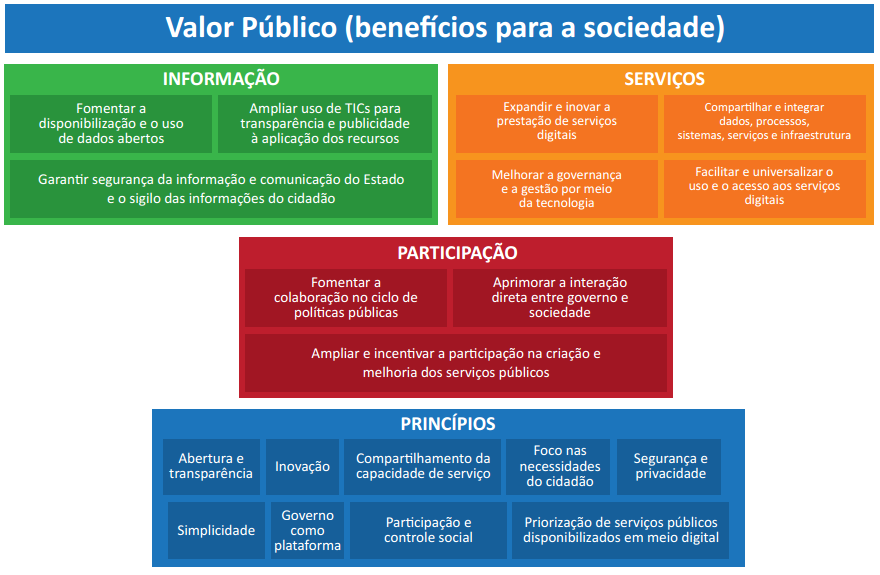
\includegraphics[width=14cm]{figuras/egdDiagramaEstrategico.png}
\caption{Diagrama estratégico da EGD, extraído de \cite{egd:16}.}
\label{figura:egdDiagramaEstrategico}
\end{figure}

Para o sucesso da EGD, os Planos Estratégicos Institucionais e os Planos Diretores de Tecnologia da Informação e Comunicação devem se alinhar aos objetivos e às iniciativas da EGD, conforme Figura \ref{figura:EGDalinhaPDTIC}. Para isto o documento recomenda aos órgãos da APF que incluam no conteúdo do PEI e do PDTIC (ou PDTI), metas e iniciativas que contribuam para o alcance dos objetivos da Estratégia de Governança Digital \cite{egd:16}.

\begin{figure}[h]
\centering % para centralizarmos a figura
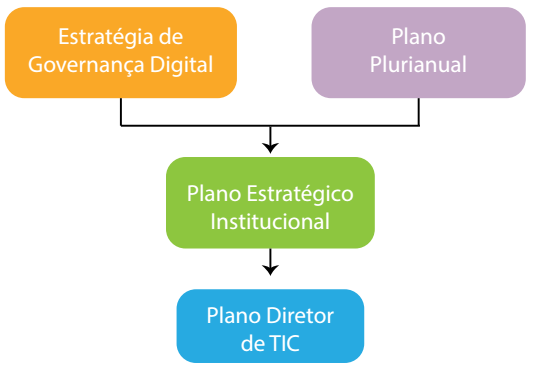
\includegraphics[width=6cm]{figuras/EGDalinhaPDTIC.png}
\caption{Integração da EGD com outras estratégias e planos, extraído de \cite{egd:16}.}
\label{figura:EGDalinhaPDTIC}
\end{figure}

O PDTIC, também chamado de PDTI, é apresentado na seção seguinte.

\subsection{PDTI}
% o que é
O planejamento de TI deve ser apresentado em um documento escrito, publicado e divulgado no âmbito da organização onde a área de TI atua \cite{sisp:12}. Para os órgãos integrantes do SISP\footnote{Sistema de Administração de Recursos de Tecnologia da Informação (SISP), organiza o planejamento, a coordenação, a organização, a operação, o controle e a supervisão dos recursos de TI dos órgãos e entidades da administração pública federal direta, autárquica e fundacional do poder executivo federal (Decreto no 7.579, de 11 de outubro de 2011).}, o planejamento de TI deve ser consolidado em um documento denominado Plano Diretor de Tecnologia da Informação. O PDTI é definido como um ``instrumento de diagnóstico, planejamento e gestão dos recursos e processos de Tecnologia da Informação que visa a atender às necessidades de informação de um órgão ou entidade para um determinado período'' \cite{in04:08,in04:10,in04:14}.

Segundo \citeonline{hazan:10}, o PDTI tem o objetivo de orientar uma organização no uso correto de seus recursos de TI, levando-a
focalizar nos processos de melhoria contínua de governança, além de atender aos princípios de racionalização, economicidade, uniformidade e padronização, criando as bases tecnológicas para a implantação com melhor eficiência e eficácia das políticas públicas. O PDTI representa um instrumento de gestão para a execução das ações e projetos de TI da organização, possibilitando justificar os recursos aplicados em TI, minimizar o desperdício e garantir o controle das atividades relacionadas à TI nos órgãos públicos da APF \cite{sisp:15}.

O PDTI ganha caráter obrigatório na IN 04/2008 quando explicita que as contratações de TI devem ser previstas no Plano: ``Art. 3º As contratações de que trata esta Instrução Normativa deverão ser precedidas de planejamento, elaborado em harmonia com o Plano Diretor de Tecnologia da Informação - PDTI, alinhado à estratégia do órgão ou entidade'' \cite{in04:08}. A existência e o uso efetivo do PDTI a partir de 2009, bem como a elaboração de um modelo de referência do Plano são abordados na primeira versão da EGTI \cite{egti:08}. 

% A inexistência de um PDTI pode causar um entendimento insuficiente do ambiente externo e interno da organização e de tecnologias emergentes que possam agregar valor aos serviços prestados aos clientes. Essa situação pode conduzir a investimentos inadequados em TI, considerando o atendimento às necessidades da organização para superar os seus desafios.  hazan:10

Considerando o caráter dinâmico do planejamento de TI devido ao fato da instabilidade dos ambientes tecnológicos, que estão em constante evolução, o PDTI deve ser anualmente revisado de forma que as estratégias estejam alinhadas à missão organizacional e à evolução da tecnologia \cite{hazan:10}.

\subsubsection{Modelos de PDTI}
%ordem cronlógica, please
Com a determinação de que os órgãos da Administração Pública Federal deveriam elaborar seus Planos Diretores de TI a partir de 2009, criou-se a necessidade de modelos e guias de orientação para a construção do PDTI. Em outubro de 2008, conforme previsto na primeira versão da EGTI, a SLTI publicou o primeiro modelo de referência de PDTI. Dividido em três fases - diagnóstico, planejamento e gestão - o modelo traz a estrutura básica do Plano. Além do modelo de referência, a SLTI propõe uma metodologia de elaboração do PDTI que será detalhada neste trabalho mais adiante.

\citeonline{fagundes:11} analisou dois modelos de PDTI aderentes à IN 04 e à EGTI naquela ocasião, em 2011, e propôs seu próprio modelo (PDGovTI). O primeiro modelo analisado por \citeonline{fagundes:11}, foi proposto pela empresa Microsoft em 2009, chamado Metodologia \textit{Microsoft Consulting Service} (MCS). O modelo tem conformidade com a IN 04, para isto segue orientações do \textit{framework} COBIT e de normas técnicas como a ISO/IEC 27002 e ISO/IEC 15999-1:2007. A metodologia MCS é distribuída sem custos para os órgãos públicos e é estruturada em cinco fases \cite{microsoft:09}:

\begin{itemize}
\item \textbf{Fase I:} Preparação e planejamento; Obter documentações; Inventariar TI; Elaborar diagnóstico de TI; Elaborar PETI.
\item \textbf{Fase II:} Pesquisar planos; Identificar setores-chave; Identificar responsáveis; Elaborar questionários de levantamento; Aplicar questionários; Consolidar levantamento de necessidades.
\item \textbf{Fase III:} Análise da situação desejada; Mapa de demandas futuras; Gerar mapa de demandas de TI.
\item \textbf{Fase IV:} Elaborar PDTI; Obter aprovação do Comitê de TI.
\item \textbf{Fase V:} Elaborar plano de execução do PDTI; Elaborar plano de monitoramento do PDTI.
\end{itemize}

O segundo modelo analisado por \citeonline{fagundes:11} também foi proposto no primeiro ano de obrigatoriedade do PDTI, em 2009. Trata-se de um modelo fornecido pela Escola Nacional de Administração Pública (ENAP) durante o curso de elaboração do PDTI de 2009. O modelo é baseado na IN 04/2008, no modelo de referência da SLTI e na EGTI \cite{cruz:08}. O modelo proposto no curso foi dividido em três etapas: preparação; diagnóstico da situação atual; planejamento da situação desejada.

Não existe uma determinação por parte do governo sobre qual modelo utilizar. Os órgãos membros do SISP são livres para seguir qualquer modelo ou criar os seus próprios, desde que atendam aos requisitos mínimos propostos na IN 04 e na EGD e, consequentemente, sejam alinhados às estratégias institucionais. Contudo, o modelo desenvolvido pela SLTI é destacado pelos órgãos membros do SISP, pois observa-se o comprometimento da SLTI em evoluir periodicamente o modelo de referência, assim como o processo de elaboração do Plano através do Guia de PDTI do SISP \cite{sisp:15}. Uma publicação que visa apoiar os órgãos a desenvolverem seus PDTI em conformidade com as normativas. Esta metodologia de elaboração do PDTI é detalhada na seção seguinte.

\subsubsection{Processo de elaboração do PDTI (Guia de PDTI do SISP)}
\label{secao:guia_pdti_sisp_cap3}
O processo de elaboração do PDTI apresentado nesta seção é descrito no Guia de PDTI do SISP, versão 2.0 beta \cite{sisp:15}. Seguindo a notação de modelagem de processos de negócio BPMN, mantida pela \textit{Object Management Group} (OMG), utiliza-se a hierarquia de elementos: macroprocessos, processos, subprocessos, atividades e tarefas.

O PDTI possui um ciclo de vida que se inicia com a criação do documento (processo de elaboração) e, após sua concepção deverá ser acompanhado ao longo de sua validade (processo de acompanhamento), realizando-se o monitoramento adequado que pode culminar em sua revisão. Um PDTI é finalizado com o término do seu período de validade e o Plano encerrado serve de insumo para o início da elaboração do Plano seguinte. Na Figura \ref{figura:pdti01Macroprocesso} é apresentado o macroprocesso do PDTI.

\begin{figure}[h!]
\centering % para centralizarmos a figura
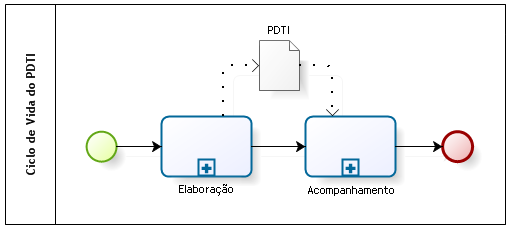
\includegraphics[width=10cm]{figuras/pdti01Macroprocesso.png}
\caption{Macroprocesso do PDTI, extraído de \cite{sisp:15}.}
\label{figura:pdti01Macroprocesso}
\end{figure}

Os principais papéis envolvidos no ciclo de vida do PDTI são:
\begin{itemize}
\item \textbf{Autoridade Máxima:} Membro da alta administração no nível hierárquico mais elevado da organização. É o principal patrocinador do PDTI e deverá prover recursos, tomar as decisões mais importantes, definir diretrizes gerais e tornar o PDTI público;
\item \textbf{Comitê de TI:} Requerido pela IN 04/2014, o comitê deve ser formado por representantes das áreas finalísticas e da TI da organização. Tem a prerrogativa de dirigir o alinhamento das ações e dos investimentos para o alcance dos objetivos estratégicos da organização, bem como priorizá-los, além de avaliar os resultados do desempenho da TI. O comitê é responsável pelo o atingimento dos objetivos e metas definidos no PDTI;
\item \textbf{Equipe de Elaboração do PDTI:} Grupo designado pelo Comitê de TI, formado por servidores tanto das áreas finalísticas quanto da TI. Equipe responsável por operacionalizar as atividades de elaboração do PDTI;
\item \textbf{Equipe de Acompanhamento do PDTI:} Equipe designada pelo Comitê de TI, responsável pelo acompanhamento do plano de ações do PDTI e pelo reporte dos resultados às partes interessadas. A equipe deve ser formada por servidores tanto das áreas finalísticas quanto da TI.
\end{itemize}

Três subprocessos compõem o processo de elaboração, sendo eles: preparação, diagnóstico e planejamento. O processo de elaboração é representado na Figura \ref{figura:pdti02Elaboracao}.
\begin{figure}[h!]
\centering % para centralizarmos a figura
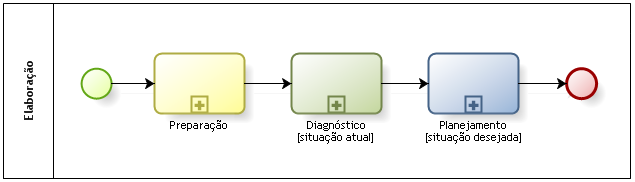
\includegraphics[width=12cm]{figuras/pdti02Elaboracao.png}
\caption{Processo de elaboração do PDTI, extraído de \cite{sisp:15}.}
\label{figura:pdti02Elaboracao}
\end{figure}

O subprocesso de preparação marca o início do processo de elaboração do PDTI. A primeira atividade consiste em definir a abrangência e o período de validade do PDTI, esta atividade deve ser realizada pelo comitê de TI. Em seguida o comitê deve definir a equipe de elaboração do PDTI e nomeá-los através de uma portaria de designação.

A primeira atividade da equipe de elaboração do PDTI no subprocesso de preparação é descrever a metodologia de elaboração do Plano. Em seguida a equipe deve produzir uma lista dos documentos de referência a serem utilizados no PDTI e listas contendo as estratégias organizacionais, princípios e diretrizes. Também é de responsabilidade da equipe de elaboração realizar nesta fase a primeira versão do inventário de necessidades. A última atividade da equipe de elaboração na fase de preparação é elaborar um plano de trabalho onde devem estar descritas as informações essenciais para organizar as atividades a serem desempenhadas durante o projeto de elaboração do PDTI. Cabe ao comitê de TI aprovar o plano de trabalho finalizando a fase de preparação.

Finalizada a preparação, inicia-se o subprocesso de diagnóstico que tem como objetivo analisar a situação atual da organização, resultando ao final do subprocesso no inventário de necessidades consolidado. Caso um PDTI necessite ser revisado, é nesta fase que a revisão deve iniciar.

Durante o diagnóstico da organização, a equipe de elaboração deve analisar os resultados do PDTI anterior, se houver; analisar o referencial estratégico de TI; analisar a organização da TI; realizar análise SWOT da TI; estimar a capacidade de execução da TI; planejar o levantamento de necessidades; identificar as necessidades de informação; identificar as necessidades de serviços, infraestrutura, contratação e pessoal de TI; consolidar o inventário de necessidades e alinhar cada necessidade de TI às estratégias da organização. Por fim, o comitê de TI aprova o inventário de necessidades finalizando a fase de diagnóstico.

Os subprocessos de preparação e diagnóstico servem de insumos para o subprocesso de planejamento, fase onde o PDTI é construído de fato. O planejamento é iniciado pelo comitê de TI com a atividade de atualização dos critérios de priorização à luz do conhecimento das necessidades levantadas anteriormente. A atividade seguinte é realizada pela equipe de elaboração e consiste na priorização das necessidades inventariadas.

Ainda no subprocesso de planejamento, a equipe de elaboração produz uma série de documentos que compõem o PDTI, sendo eles: Plano de Metas e Ações; Plano de Gestão de Pessoas; Plano Orçamentário; Lista dos fatores críticos de sucesso; Plano de Gestão de Riscos. A equipe de elaboração do PDTI encerra sua participação nesta fase consolidando uma minuta do PDTI que segue para a aprovação do comitê de TI e, por fim, para a autoridade máxima realizar a atividade de publicação do Plano. Desta forma o processo de elaboração do PDTI é finalizado. Todo o subprocesso de planejamento é ilustrado na Figura \ref{figura:pdti04Planejamento}.
\begin{figure}[h!]
\centering % para centralizarmos a figura
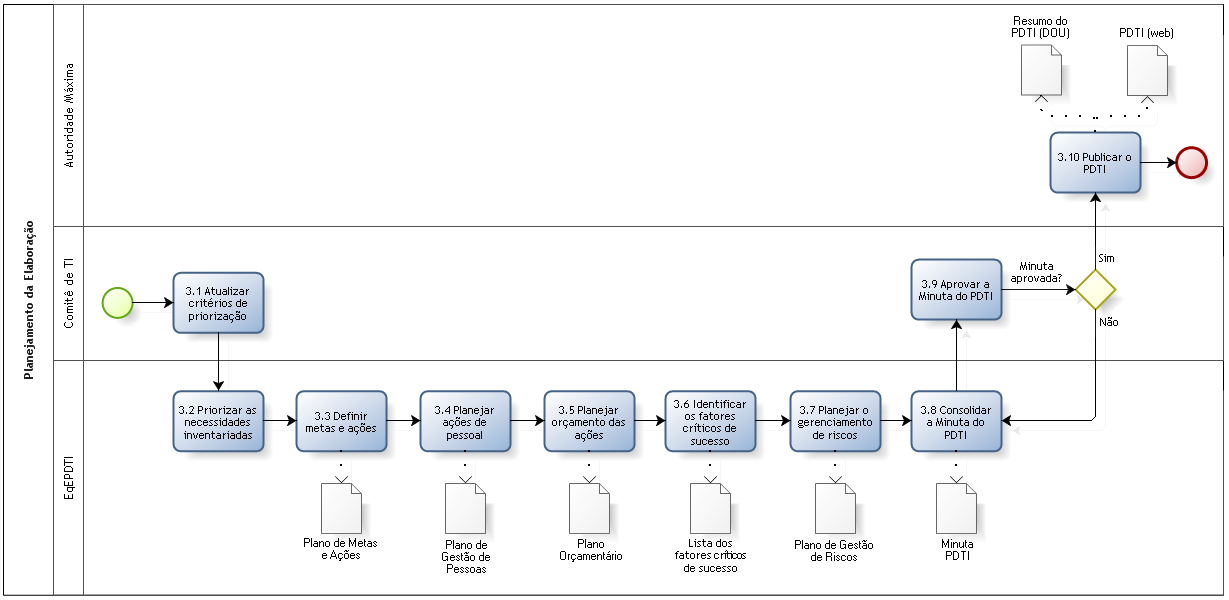
\includegraphics[width=16cm]{figuras/pdti04Planejamento.png}
\caption{Subprocesso de planejamento do PDTI, extraído de \cite{sisp:15}.}
\label{figura:pdti04Planejamento}
\end{figure}

\section{Trabalhos Relacionados}

%oportunidade de usar o trabalho de outros autores para motivar o seu próprio estudo

Inicialmente, é importante destacar que não há o objetivo de realizar um mapeamento sistemático da literatura neste trabalho. O intuito desta seção é apresentar trabalhos com temática diretamente relacionada a esta pesquisa. Os resultados das buscas por trabalhos relacionados foram classificados por relevância e selecionados informalmente, priorizando trabalhos recentes e com abordagens correlatas ao problema de pesquisa aqui apresentado.

Para buscar trabalhos relacionados ao tema foi utilizado o engenho de busca contido no Portal de Periódicos da CAPES, além da base de teses e dissertações. A Tabela \ref{tabela:stringsIngles} apresenta as \textit{strings} utilizadas nas buscas em língua inglesa e a Tabela \ref{tabela:stringsPortugues} apresenta as \textit{strings} utilizadas nas buscas em língua portuguesa. As buscas limitaram-se a trabalhos dos últimos seis anos, de 2011 a 2016.

% http://www.tablesgenerator.com/
% Please add the following required packages to your document preamble:
% \usepackage[table,xcdraw]{xcolor}
% If you use beamer only pass "xcolor=table" option, i.e. \documentclass[xcolor=table]{beamer}
\begin{table}[h!]
\centering
\begin{tabular}{|l|c|c|}
\hline
\rowcolor[HTML]{9B9B9B} 
\multicolumn{1}{|c|}{\cellcolor[HTML]{9B9B9B}{\color[HTML]{000000} \textit{\textbf{String}}}}                                    & {\color[HTML]{000000} \textbf{\begin{tabular}[c]{@{}c@{}}Trabalhos \\ retornados\end{tabular}}} & {\color[HTML]{000000} \textbf{\begin{tabular}[c]{@{}c@{}}Trabalhos\\ selecionados\end{tabular}}} \\ \hline
"IT Planning" (título)                                                                                                           & 7                                                                                               & 0                                                                                                \\ \hline
"Information Techonology Planning" (título)                                                                                      & 0                                                                                               & 0                                                                                                \\ \hline
\begin{tabular}[c]{@{}l@{}}"IT Planning" (título) AND \\ "government" (documento todo)\end{tabular}                              & 3                                                                                               & 0                                                                                                \\ \hline
\begin{tabular}[c]{@{}l@{}}"IT Planning" (título) AND \\ "Public Sector" (documento todo)\end{tabular}                           & 1                                                                                               & 0                                                                                                \\ \hline
"Strategic Information Systems Planning" (título)                                                                                & 15                                                                                              & 0                                                                                                \\ \hline
\begin{tabular}[c]{@{}l@{}}"Strategic Information Systems Planning" (título) \\ AND "government" (documento todo)\end{tabular}   & 5                                                                                               & 0                                                                                                \\ \hline
\begin{tabular}[c]{@{}l@{}}"Strategic Information Systems Planning" (título)\\ AND "public sector" (documento todo)\end{tabular} & 2                                                                                               & 0                                                                                                \\ \hline
\end{tabular}
\caption{\textit{Strings} de busca em periódicos na língua inglesa }
\label{tabela:stringsIngles}
\end{table}


% Please add the following required packages to your document preamble:
% \usepackage[table,xcdraw]{xcolor}
% If you use beamer only pass "xcolor=table" option, i.e. \documentclass[xcolor=table]{beamer}
\begin{table}[h!]
\centering
\begin{tabular}{|l|c|c|}
\hline
\rowcolor[HTML]{9B9B9B} 
\multicolumn{1}{|c|}{\cellcolor[HTML]{9B9B9B}{\color[HTML]{000000} \textit{\textbf{String}}}} & {\color[HTML]{000000} \textbf{\begin{tabular}[c]{@{}c@{}}Trabalhos \\ retornados\end{tabular}}} & {\color[HTML]{000000} \textbf{\begin{tabular}[c]{@{}c@{}}Trabalhos\\ selecionados\end{tabular}}} \\ \hline
"Planejamento de TI" (título) & 0 & 0 \\ \hline
"Planejamento de tecnologia da informação" (título) & 4 & 0 \\ \hline
"PDTI" (título) & 1 & 0 \\ \hline
"Plano diretor de TI" (título) & 1 & 0 \\ \hline
"Plano de TI" (título) & 0 & 0 \\ \hline
"Planos de TI" (título) & 1 & 1 \\ \hline
"Planejamento estratégico de TI" (título) & 13 & 0 \\ \hline
"Planejamento estratégico de\\ Tecnologia da Informação" (título) & 5 & 2 \\ \hline
\end{tabular}
\caption{\textit{Strings} de busca em trabalhos na língua portuguesa}
\label{tabela:stringsPortugues}
\end{table}

As buscas por trabalhos relacionados revelaram que a maior parte das produções acadêmicas sobre planejamento de TI se referem ao setor privado. Nos trabalhos mais recentes, das poucas publicações que abordam o planejamento de TI no setor público brasileiro a grande maioria são teses ou dissertações. O contrário ocorre com as publicações em língua inglesa, onde percebe-se que as publicações que abordam planejamento de TI no setor público são artigos de periódicos e conferências.

Na seleção dos trabalhos, o principal critério consistiu na relação entre o planejamento de TI e setor público. Posteriormente, foram filtrados apenas trabalhos focados em planejamentos de TI de organizações públicas brasileiras cujo escopo contribuísse para a presente pesquisa. Os três trabalhos relacionados são dissertações de mestrado: \citeonline{paula:12}; \citeonline{barros:13}; \citeonline{prando:15}.

\subsection{Fatores condicionantes relacionados ao planejamento de TI}
% do problema de pesquisa
A caracterização do problema na dissertação de \citeonline{paula:12} evidencia que naquela ocasião já era visível que, apesar da obrigatoriedade de realizar o planejamento de TI, os órgãos públicos brasileiros encontravam dificuldades para realizar tal atividade. Diante disso, \citeonline{paula:12} pesquisou sobre modelos de planejamento de TI aderentes ao setor público. Ao investigar as práticas de formulação e implantação do planejamento de TI em órgãos federais, \citeonline{barros:13} identificou fatores condicionantes que se relacionam com a formulação e implantação de planos de TI. No trabalho de \citeonline{prando:15}, um dos objetivos consiste em explorar as lacunas e conflitos presentes no processo de planejamento de TI de uma instituição pública federal em um cenário de expansão.

%dos fatores que dificultam o planejamento

\citeonline{paula:12} utilizou-se da literatura científica para levantar a hipótese de sua pesquisa. Nesta abordagem, a falta de um modelo de formulação de planejamento estratégico de TI voltado para instituições universitárias federais, seria o fator restritivo para que estas instituições atendessem satisfatoriamente o planejamento de TI. 

Para identificar os fatores condicionantes que influem na elaboração e execução dos planos de TI de órgãos públicos federais, \citeonline{barros:13} entrevistou dirigentes de TI codificando seus depoimentos de acordo com as categorias do modelo teórico de \citeonline{brown:04}. Desta forma, o autor organizou as percepções dos entrevistados a respeito do planejamento de TI sob a perspectiva das dez categorias do trabalho de \citeonline{brown:04}, que por sua vez, foram mapeadas a partir da literatura científica.

No trabalho de \citeonline{prando:15}, a pesquisa baseou-se em cinco proposições acerca das dificuldades relacionadas à elaboração do PDTI em uma determinada instituição. As proposições foram expostas à validação através de pesquisa documental, entrevistas e estudo de caso.

Um dos objetivos da presente pesquisa é identificar os fatores que dificultam ou impedem a elaboração do planejamento de TI em órgãos públicos federais. Desta forma, com o intuito de realizar comparações a Tabela \ref{tabela:fatoresTrabRelacionados} foi elaborada compilando os principais fatores que dificultam o planejamento de TI, sob a perspectiva de cada trabalho relacionado neste capítulo.

% Please add the following required packages to your document preamble:
% \usepackage{graphicx}
% \usepackage[table,xcdraw]{xcolor}
% If you use beamer only pass "xcolor=table" option, i.e. \documentclass[xcolor=table]{beamer}
\begin{table}[h!]
\centering
\resizebox{\textwidth}{!}{%
\begin{tabular}{|l|l|l|}
\hline
\rowcolor[HTML]{9B9B9B} 
\multicolumn{1}{|c|}{\cellcolor[HTML]{9B9B9B}{\color[HTML]{000000} Paula (2012)}}                                                      & \multicolumn{1}{c|}{\cellcolor[HTML]{9B9B9B}{\color[HTML]{000000} Barros (2013)}}                                                                                                                                                                                                                                                                                                                                                                                                                                                                                                                                                                                                                                                              & \multicolumn{1}{c|}{\cellcolor[HTML]{9B9B9B}{\color[HTML]{000000} Prando (2015)}}                                                                                                                                                                                                                                       \\ \hline
\begin{tabular}[c]{@{}l@{}}- Dificuldade em aplicar modelos de \\ planejamento de TI no cenário de instituição\\ pública.\end{tabular} & \begin{tabular}[c]{@{}l@{}}- Influência (negativa) da alta gestão;\\ - Mudanças no cenário político impedem o planejamento\\  a longo prazo;\\ - Contingenciamento orçamentário;\\ - Dificuldade em consolidar as informações de todas as \\ áreas em instituições com grande número de unidades;\\ - Rotatividade de dirigentes e descontinuidade \\ administrativa;\\ - Falta de governança corporativa;\\ - Falta de cultura de planejamento e de pensamento \\ estratégico;\\ - TI mal posicionada na hierarquia organizacional;\\ - Falta pessoal de TI;\\ - Falta qualificação do quadro de pessoal;\\ - Dificuldades para conseguir a participação das áreas\\ finalísticas;\\ - Dificuldades na priorização das demandas.\end{tabular} & \begin{tabular}[c]{@{}l@{}}- Expansão acelerada da instituição;\\ - Parte dos coordenadores de TI desconhecem\\ o PDTI;\\ - Alinhamento estratégico fraco ou inexistente;\\ - Coordenadores de TI há pouco tempo no cargo;\\ - Dificuldade em manter o comprometimento\\ dos participantes do comitê de TI.\end{tabular} \\ \hline
\end{tabular}%
}
\caption{Fatores que dificultam o planejamento de TI, segundo trabalhos relacionados.}
\label{tabela:fatoresTrabRelacionados}
\end{table}

Pode-se observar que dificuldades em aplicar modelos de planejamento de TI no setor público, como coloca \citeonline{paula:12}, não é um fator que aparece na teoria fundamentada nos dados apresentada nesta pesquisa. Isto permite inferir que os processos, guias e ferramentas disponíveis nas instituições pesquisadas não se apresentaram como dificuldade na elaboração do planejamento de TI.

Dos fatores citados no trabalho de \citeonline{barros:13} é possível observar que a influência (negativa) da alta gestão está presente nas duas teorias fundamentadas nos dados, assim como as deficiências de capacitação e quantitativas do pessoal de TI. A falta da cultura do planejamento, citada pelo autor, se faz presente na teoria 2 da presente pesquisa. Também foi citado por \citeonline{barros:13} o elemento centra da teoria 2: dificuldades com a participação das áreas finalísticas; desta forma corroborando com a teoria apresentada. Contudo, vários fatores citados pelo autor não se mostraram presentes nas teorias desta pesquisa, tais como: mudanças no cenário político, contingenciamento orçamentário, dificuldade em consolidar informações das unidades, rotatividade de dirigentes e dificuldade em priorizar as demandas.

Já no trabalho de \citeonline{prando:15} não foi possível traçar nenhuma relação direta entre os fatores levantados pelo autor e os elementos das teorias desta pesquisa. Porém, é possível inferir que há alguma relação entre o elemento central da teoria 2 (problemas na participação das áreas de negócio) com a dificuldade em manter o comprometimento dos participantes do comitê de TI, citado por \citeonline{prando:15}, uma vez que o comitê de TI deve conter membros de variadas áreas da instituição.

De forma geral, com exceção do trabalho de \citeonline{paula:12}, foi possível verificar que os trabalhos relacionados apontam para fatores condicionantes ao planejamento de TI de forma específica e pontual. As teorias apresentadas nesta pesquisa, conforme determina \citeonline{corbin:98}, são abrangentes o suficientes para englobar tais especifidades e se mostrou aderente em diversos fatores levantados nos trabalhos relacionados. Por outro lado, a teoria fundamentada nos dados desta pesquisa não revelou convergência com a maioria dos fatores listados pelos trabalhos relacionados apresentados nesta seção. Infere-se que os métodos de cada pesquisa possam influir nesta divergência parcial.

\subsection{Métodos utilizados}
Os métodos empregados em cada trabalho relacionado neste capítulo também contribuíram para a presente pesquisa. O intuito desta seção é destacar a metodologia de cada pesquisa para poder comparar os trabalhos e interpretar os resultados de forma ponderada. Desta maneira, não é objeto desta seção descrever os métodos, mas espera-se expor as características relevantes na influência dos resultados e suas análises.

\citeonline{paula:12} utilizou o método pesquisa-ação, que pode ser definida como ``toda tentativa continuada, sistemática e empiricamente fundamentada de aprimirar a prática'' \cite{tripp:05}. Neste cenário, a prática envolvida consiste na formulação do planejamento estratégico de TI de uma determinada instituição. A pesquisa-ação desenvolveu-se em três etapas: planejar, agir e refletir.

\begin{citacao}
Na etapa planejar, foi realizada a avaliação dos fatores que influenciam o planejamento estratégico de TI na UNIRIO e a análise dos modelos de planejamento estratégico de TI existentes na literatura. Na etapa Agir foi aplicado o Modelo de Planejamento Estratégico de TI desenvolvido pelo SISP, tendo como resultado o PDTIC da UNIRIO. Na etapa Refletir, foram apresentadas as reflexões sobre os efeitos decorrentes da aplicação da modelo do SISP e a identificação de possíveis melhorias para futuros ciclos de planejamento \cite{paula:12}.
\end{citacao}

No método utilizado por \citeonline{paula:12}, destaca-se a fase ``planejar'', na qual avaliou-se os fatores que influenciam o planejamento de TI da instituição. A autora confirmou seu problema de pesquisa nesta etapa ao traçar o cenário da instituição com relação ao planejamento de TI. Para isto, analisou o histórico da instituição; buscou a origem do problema de planejamento de TI estabelecendo contato com os participantes e interessados. Há de se destacar que a pesquisadora interferiu no ambiente da pesquisa por ser membro do comitê de TI da instituição pesquisada. Porém, o método utilizado permite tal interferência. Traçando um comparativo com a metodologia da presente pesquisa, a interferência do pesquisador não é bem-vinda, pois pode-se distanciar os dados da realidade e aproximá-los do viés do pesquisador.

A pesquisa de \citeonline{barros:13} é de natureza qualitativa, aplicando entrevistas semiestruturadas à alguns dirigentes de TI de organizações públicas federais. Os dados coletados são codificados de acordo com as categorias pré-concebidas no modelo teórico de \citeonline{brown:04}, ou seja, possui traços de \textit{Grounded Theory}. Desta forma, o pesquisador não apresenta uma teoria fundamentada nos dados, assim como foi apresentado no presente trabalho, mas uma classificação de códigos de acordo com um modelo teórico fundamentado na literatura.

\citeonline{prando:15} também optou pela abordagem qualitativa, porém utilizando os métodos de estudo de caso, entrevistas em profundidade e pesquisa documental. Tal metodologia permitiu ao pesquisador traçar o retrato fiel da instituição pesquisada e propor recomendações direcionadas aos problemas levantados. Porém, esta abordagem restringe a generalização do problema para outras instituições, uma vez que os fatores condicionantes levantados são de natureza específica da instituição em questão.

\subsection{Soluções propostas}
O trabalho de \citeonline{paula:12} permitiu a adaptação de um modelo de planejamento de TI existente, gerando um modelo exclusivo voltado para atender à instituição pesquisada. Desta forma, a pesquisadora buscou eliminar as lacunas e dificuldades que a instituição enfrentava no processo de elaboração do PDTI. Contudo, o contexto de outras instituições pode ser diferente e, com isto, o modelo proposto pode não ser aplicável.

A proposta de \citeonline{barros:13} é explorar a perspectiva dos dirigentes de TI e expor os fatores que influenciam a formulação e execução dos planos de TI. Os relatos dos dirigentes são ricos e o pesquisador os apresenta de forma a mostrar contrapontos e justificativas dos entrevistados. Porém, apesar de levantar os fatores condicionantes à elaboração do planejamento de TI, o trabalho não fornece uma proposta soluções aos problemas relacionados ao planejamento de TI. Ao contrário, a presente pesquisa propõe um conjunto de melhores práticas relacionadas aos fatores condicionantes.

A pesquisa de \citeonline{prando:15} oferece um conjunto de recomendações com o intuito de reduzir os problemas levantados. O autor não especifica a fonte das recomendações, desta forma infere-se que as sugestões foram baseadas no conhecimento do próprio autor. Por se tratar de uma pesquisa com foco específico em problemas de planejamento de TI de uma determinada instituição, fica dificultada a generalização das recomendações propostas e, consequentemente, a aplicação em outras instituições. As teorias apresentadas na presente pesquisa vão de encontro à abordagem de \citeonline{prando:15}, uma vez que apresenta uma teoria substancial e geral, além de apresentar uma proposta de solução com fundamentação nos dados.

\subsection{Considerações}
Os três trabalhos relacionados corroboram com a motivação da presente pesquisa fornecendo diferentes abordagens de identificação das dificuldades e deficiências no planejamento de TI de organizações públicas e propondo ações de melhoria para o cenário pesquisado.

A proposta da presente pesquisa, ao utilizar \textit{Grounded Theory}, não utilizou-se de premissas ou hipóteses assim como nos trabalhos de \citeonline{paula:12} e \citeonline{prando:15}. Ao contrário, as proposições foram levantadas na análise dos dados coletados e refutadas ou confirmadas também nos dados no desenvolver da pesquisa.

É interessante observar que \citeonline{barros:13} utilizou \textit{Grounded Theory} de forma indireta em sua pesquisa. Isto pode ser afirmado pois o autor codifica os dados utilizando categorias mapeadas anteriormente por \citeonline{brown:04}, que utilizaram GT para formular tal modelo. A criação das categorias da presente pesquisa foi feita de forma diferente, pois foram mapeadas a partir dos dados coletados exclusivamente para esta pesquisa, contribuindo para a fundamentação das teorias descobertas.

Os três trabalhos apresentados nesta pesquisa comungam de um problema prático presente nas instituições públicas brasileiras: as dificuldades em se planejar de forma eficaz as ações de TI de uma organização pública. As pesquisas aqui apresentadas apontam que a busca pela identificação dos fatores que levam a este problema é uma tarefa complexa e subjetiva. Porém, não atenderam a necessidade de compreender de forma abrangente os fatores limitadores do planejamento de TI e expor as relações causais entre estes limitadores. Tal lacuna foi sanada na presente pesquisa com duas teorias substanciais e abrangentes, ou seja, com fundamentação e genéricas o suficiente para aplicação em diversas organizações. A fundamentação empírica desta pesquisa é um diferencial para que a teoria reflita diretamente a prática, permitindo a proposição de soluções eficazes.

Por fim, esta pesquisa difere-se dos trabalhos relacionados também na proposta de solução do problema de planejamento de TI no setor público brasileiro. Apresentou-se as melhores práticas de planejamento estratégico de TI cujos resultados esperados atacam diretamente os elementos causais do problema pesquisado. Destaca-se ainda a utilização do método GT na fase de seleção das melhores práticas, mantendo o rigor científico e a fundamentação teórica da pesquisa.

%Porém, compreender a origem do problema é um passo necessário para propor as soluções.


\section{Considerações}
Este capítulo apresentou as bases teóricas sobre o alinhamento estratégico entre a TI e o negócio e sobre os principais instrumentos de planejamento de TI. Destacam-se as particularidades do planejamento de TI no setor público, além dos fatos e normativas que motivaram a evolução da gestão de TI nos órgãos públicos federais brasileiros.

Assim como no setor privado, existem diversos modelos de planejamento de TI para o setor público. É importante destacar o esforço que o governo federal têm feito, através da SLTI e dos órgãos da APF que compõem o SISP, ao desenvolver instrumentos como a Instrução Normativa número 4, a Estratégia Geral de TI e a Estratégia Geral Digital no intuito de prover as bases estratégicas para o amadurecimento da TI no âmbito do setor público.

O processo de elaboração do PDTI apresentado neste capítulo é utilizado por grande parte dos órgãos da APF e suas etapas serviram de insumo para a composição do questionário aplicado à amostragem de entes da administração pública durante esta pesquisa. 

Com o intuito de explorar a literatura científica sob à temática do planejamento de TI no setor público, o capítulo seguinte apresenta os trabalhos relacionados que possuem relevância no desenvolvimento da presente pesquisa.